\documentclass[a4paper,oneside,12pt]{book}
%% === nezbytné balíčky:
\usepackage[IL2]{fontenc}   % písmo pro UTF-8 || jiné: [T1] (funguje pro UTF-8?)
\usepackage[utf8]{inputenc} % vstupní znaková sada UTF-8 || [cp1250] -> Windows 1250 || [latin2] -> ISO Latin 2
\usepackage{float}
\usepackage[czech]{babel} % česky psaná práce, typografická pravidla     

\usepackage{pdfpages} % pokud nemáte formulář "Zadání bak./dipl. práce" naskenovaný jako PDF, tak ZAKOMENTUJTE

%\usepackage{encxvlna} % postará se o spojky a předložky, které dle českých pravidel nesmí být na konci řádku. Dokumentace: http://texdoc.net/texmf-dist/doc/generic/encxvlna/encxvlna.pdf

\usepackage[a4paper, hmarginratio=1:1]{geometry} % využití celé A4 stránky a nastavení okrajů, pro OBOUSTRANNÝ TISK

%% === balíčky, které se mohou hodit:
\usepackage[hidelinks]{hyperref} % v PDF budou klikací odkazy ("hidelinks" je nebude rámovat)
\usepackage{graphicx} % balíček pro vkládání RASTROVÝCH grafických souborů (PNG apod.)
%\usepackage{epsfig} % balíčky pro vkládání VEKTOROVÝCH grafických souborů typu EPS

%\usepackage{float} % rozšířené možnosti umístění obrázků
%\usepackage{caption} % pro popisky obrázků, tabulek atd.

\usepackage{tabularx} % rozšířené možnosti tabulek
%\usepackage{tabu} % jiný balík pro rozšířené možnosti tabulek

\usepackage{listings}  % balíček vhodný pro ukázky kódu 
\usepackage{amsmath} % balíček pro pokročilou matematickou sazbu
%\usepackage{color} % pro možnost barevného textu
%\usepackage{fancybox} % umožňuje pokročilé rámečkování
%\usepackage{index} % nutno použít v případě tvorby rejstříku balíčkem makeindex
%\newindex{default}{idx}{ind}{Rejstřík} % zavádí rejstřík v případě použití balíku index


\topmargin=-15mm      % horní okraj trochu menší
\textwidth=150mm      % šířka textu na stránce
\textheight=240mm     % "výška" textu na stránce

\frenchspacing % za větou bude mezislovní mezera (v anglických textech je mezera za větou delší)
\widowpenalty=1000 % "síla" zákazu vdov (= jeden řádek odstavce na konci stránky)
\clubpenalty=1000 % "síla" zákazu sirotků (= jeden řádek/slovo odstavce samostatně na začátku stránky)
\brokenpenalty=1000 % "síla" zákazu zlomu stránky za řádkem, který má na konci rozdělené slovo

\pagenumbering{arabic} % číslování stránek arabskými číslicemi
\pagestyle{plain}      % stránky číslované dole uprostřed

\parindent=0pt % odsazení 1. řádku odstavce
\parskip=7pt   % mezera mezi odstavci

\newcommand{\ti}{\textit} % zkrácený příkaz pro kurzívu
\newcommand{\tb}{\textbf} % zkrácený příkaz pro tučné písmo


%% --- zde jsou makra, tj. "konstanty" - některé musíte změnit! --- %%
\newcommand{\cvut}{České vysoké učení technické v~Praze}
\newcommand{\fjfi}{Fakulta jaderná a fyzikálně inženýrská}
\newcommand{\katedra}{Katedra softwarového inženýrství}
\newcommand{\program}{Aplikace informatiky v~přírodních vědách} % změňte, pokud máte jiný stud. program
\newcommand{\spec}{--} % změňte, pokud studijní program má specializaci

\newcommand{\druh}{Bakalářská práce} % nebo "Diplomová práce"
\newcommand{\woman}{} % pokud jste ŽENA, ZMĚŇTE na: ...{\woman}{a} (je to do Prohlášení)

\newcommand{\logoCVUT}{
\includegraphics{symbol_cvut_konturova_verze_cb.pdf}} % logo ČVUT -- podle grafického manuálu ČVUT platného od prosince 2016. Pokud nevyhovuje PDF-verze, tak použijte jinou variantu loga: https://www.cvut.cz/logo-a-graficky-manual -> "Symbol a logo ČVUT v Praze"). Pokud chcete logo úplně vynechat, zadejte místo "\includegraphics{...}" text "\vspace{35mm}"

% přesně podle formuláře "Zadání bak./dipl. práce" VYPLŇTE:
\newcommand{\nazevcz}{Využití metod virtuální reality pro vizualizaci numerické simulace dynamiky tekutin}    % český název práce (přesně podle zadání!)
\newcommand{\nazeven}{Utilization of virtual reality tool for the visualization of fluid flow numerical simulation}          % anglický název práce (přesně podle zadání!)
\newcommand{\autor}{Martin Tůma}   % vyplňte své jméno a příjmení (s akademickým titulem, máte-li jej)
\newcommand{\vedouci}{Ing. Pavel Eichler, Ph.D.} % vyplňte jméno a příjmení vedoucího práce, včetně titulů, např.: Doc. Ing. Ivo Malý, Ph.D.
\newcommand{\pracovisteVed}{\katedra, \fjfi, \cvut} % ZMĚŇTE, pokud vedoucí Vaší práce není z KSI
\newcommand{\konzultant}{--} % POKUD MÁTE určeného konzultanta, NAPIŠTE jeho jméno a příjmení + tituly
\newcommand{\pracovisteKonz}{--} % POKUD MÁTE konzultanta, NAPIŠTE jeho pracoviště

% podle skutečnosti VYPLŇTE:
\newcommand{\rok}{2025}  % rok odevzdání práce (jen rok odevzdání, nikoli celý akademický rok!)
\newcommand{\kde}{Děčíně} % studenti z Děčína ZMĚNÍ na: "Děčíně" (doplní se k "prohlášení")

\newcommand{\klicova}{Virtuální realita}   % zde NAPIŠTE česky cca 3-5 klíčových slov
\newcommand{\keyword}{Virtual reality}       % zde NAPIŠTE anglicky cca 3-5 klíčových slov (přeložte z češtiny, ale odborně)
\newcommand{\abstrCZ}{Popis práce česky}    % zde NAPIŠTE abstrakt v češtině (alespoň 7 vět, min. 80 slov. Pokuste se, aby CZ i EN abstrakt nezpůsobily přetečení strany 6 na stranu 7, tj. aby se obojí i s klíčovými slovy vešlo na JEDNU stránku)
\newcommand{\abstrEN}{Popis práce anglicky} % zde NAPIŠTE abstrakt v angličtině

\newcommand{\prohlaseni}{Prohlašuji, že jsem svou bakalářskou práci vypracoval\woman{} samostatně a použil\woman{} jsem pouze podklady (literaturu, projekty, SW atd.) uvedené v přiloženém seznamu.} % text prohlášení můžete mírně upravit :-)

\newcommand{\podekovani}{Děkuji ... za ...} % NAPIŠTE poděkování, např. svému vedoucímu:
%"Děkuji Ing. Eleonoře Krtečkové, Ph.D. za vedení mé bakalářské práce a za podnětné návrhy, které ji obohatily."
% NEBO:
% Děkuji vedoucímu práce doc. Ing. Pafnutijovi Snědldítětikaši, Ph.D. za neocenitelné rady a pomoc při tvorbě bakalářské práce.


\begin{document}
%%%%%%%%%%%% TITULNÍ STRANA -- následujících cca 30 řádků se generuje AUTOMATICKY. Neměňte!!! Výjimka: práce psané v angličtině! %%%%%%%%%%%%
\thispagestyle{empty}

\begin{center}
    {\Large \textsc{\cvut}\\[4mm] \textsc{\fjfi}}\par
    \vspace{4mm}
	\tb{\katedra} \par\vspace{3mm}

    \begin{tabular}{l}
		\tb{Studijní program: \program}\\
    \end{tabular}

   \vspace{10mm} \logoCVUT \vspace{15mm} 

   {\huge \tb{\nazevcz}\par}
   \vspace{5mm}   
   {\huge \tb{\nazeven}\par}
   
   \vspace{15mm}
   {\Large \MakeUppercase{\druh}}

   \vfill
   {\large
    \begin{tabular}{ll}
    Vypracoval: & \autor\\
    Vedoucí práce: & \vedouci\\
    Rok: & \rok
    \end{tabular}
   }
\end{center}

%%%%%%%%%%%% ZADÁNÍ PRÁCE %%%%%%%%%%%%
% Zadání (podepsané děkanem atd.) dostanou studenti KSI od sekretářky (nebo ji požádají, např. e-mailem).
\newpage  % SEM NESAHEJTE!
\thispagestyle{empty} % SEM NESAHEJTE!

%% naskenované ZADÁNÍ PRÁCE (nechte odkomentovanou jednu možnost!):
%% --- varianta A1: jednostránkové zadání v PDF:
%\includepdf[pages={1}]{zadani_cele.pdf} % A1) naskenováno do PDF
%% --- varianta A2: jednostránkové zadání v JPG:
%\begin{center}
%     \includegraphics[width=1\textwidth]{zadani1.jpg}
%\end{center}
%% --- varianta B1: dvoustránkové zadání v jediném PDF:



% ---------------- TADY PDF ZADANI
%\includepdf[pages={1,2}]{zadani_cele.pdf} % PDF má 2 stránky



%% --- varianta B2: dvoustránkové zadání naskenované jako dvě samostatná jednostránková PDF:
%\includepdf[pages={1}]{zadani1.pdf} % 1. strana zadání v PDF
%\includepdf[pages={1}]{zadani2.pdf} % 2. strana zadání v PDF
%% --- varianta B3: dvoustránkové zadání naskenované jako dva samostatné JPG:
%\begin{center}
%     \includegraphics[width=1\textwidth]{zadani1.jpg} % 1. strana zadání
%\end{center}
%\newpage  
%\thispagestyle{empty}
%\begin{center}
%     \includegraphics[width=1\textwidth]{zadani2.jpg} % 2. strana zadání
%\end{center}
%% --- konec varianty B3


%%%%%%%%%%%% Prohlášení -- SEM NESAHEJTE! Generuje se automaticky z výše nastavených maker \kde{} a \prohlaseni{}. %%%%%%%%%%%%
\newpage % SEM NESAHEJTE!
\thispagestyle{empty}  % SEM NESAHEJTE!

~ % SEM NESAHEJTE!
\vfill % prázdné místo. SEM NESAHEJTE!

\tb{Prohlášení} % SEM NESAHEJTE!

\vspace{1em} % vertikální mezera. SEM NESAHEJTE!
\prohlaseni

\vspace{2em}  % SEM NESAHEJTE!
\hspace{-0.5em}\begin{tabularx}{\textwidth}{X c}  % SEM NESAHEJTE!
V \kde\ dne .................... &........................................ \\	% SEM NESAHEJTE!
	& \autor
\end{tabularx}	% SEM NESAHEJTE!


%%%%%%%%%%%% Poděkování -- tuto stránku můžete celou odstranit %%%%%%%%%%%%
%\newpage
%\thispagestyle{empty}

%~
%\vfill % prázdné místo

%\tb{Poděkování}

%\vspace{1em} % vertikální mezera
%\podekovani
%\begin{flushright}
%\autor
%\end{flushright}  % <------- tady končí stránka s poděkováním


%%%%%%%%%%%% ABSTRAKT atp. Je generován AUTOMATICKY podle maker nastavených na začátku souboru) %%%%%%%%%%%% 
\newpage   % SEM NESAHEJTE!
\thispagestyle{empty}   % SEM NESAHEJTE!

% příprava:    (na následujících 8 řádků NESAHEJTE!)
\newbox\odstavecbox
\newlength\vyskaodstavce
\newcommand\odstavec[2]{%
    \setbox\odstavecbox=\hbox{%
         \parbox[t]{#1}{#2\vrule width 0pt depth 4pt}}%
    \global\vyskaodstavce=\dp\odstavecbox
    \box\odstavecbox}
\newcommand{\delka}{120mm} % šířka textů ve 2. sloupci tabulky

% použití přípravy:    % dovnitř "tabular" vůbec NESAHEJTE!
\begin{tabular}{ll}
  {\em Název práce:} & ~ \\
  \multicolumn{2}{l}{\odstavec{\textwidth}{\bf \nazevcz}} \\[1em]
  {\em Autor:} & \autor \\[1em]
  {\em Studijní program:} & \program \\
  {\em Specializace:} & \spec \\
  {\em Druh práce:} & \druh \\[1em]
  {\em Vedoucí práce:} & \odstavec{\delka}{\vedouci\\ \pracovisteVed} \\
  {\em Konzultant:} & -- %\odstavec{\delka}{\konzultant \\ \pracovisteKonz}  % VYMAŽTE text "-- %" v případě, že jste neměli konzultanta
 \\[1em]  
  \multicolumn{2}{l}{\odstavec{\textwidth}{{\em Abstrakt:} ~ \abstrCZ  }} \\[1em]
  {\em Klíčová slova:} & \odstavec{\delka}{\klicova} \\[2em]

  {\em Title:} & ~\\
  \multicolumn{2}{l}{\odstavec{\textwidth}{\bf \nazeven}}\\[1em]
  {\em Author:} & \autor \\[1em]
  \multicolumn{2}{l}{\odstavec{\textwidth}{{\em Abstract:} ~ \abstrEN  }} \\[1em]
  {\em Key words:} & \odstavec{\delka}{\keyword}
\end{tabular}



%%%%%%%%%%%% Obsah práce ... je generován AUTOMATICKY %%%%%%%%%%%%
\newpage  % SEM NESAHEJTE!
\parskip=0pt
\tableofcontents % SEM NESAHEJTE!
\parskip=7pt
\newpage % SEM NESAHEJTE!


%--------------------------------------------------------
%|         Zde začíná SAMOTNÁ PRÁCE (text)              |
%--------------------------------------------------------




\chapter*{Úvod} % SEM NESAHEJTE!
\addcontentsline{toc}{chapter}{Úvod} % SEM NESAHEJTE!
%
S technologickým vývojem se objevila z různých specializovaných důvodů potřeba manipulovat s daty ve 3-rozměrném prostoru a tak byly vyvinuté technologie, které toto zobrazení umožňují. Mezi tyto technologie patří VR (Virtual Reality), AR (Augmented Reality) a MR (Mixed Reality). VR je technologie která nám umožňuje vstoupit do digitálního světa a manipulovat s 3D objekty, AR zachovává prvky opravdového světa a přidává k němu digitální "displej" (představme si například jako HUD v herním světě). MR se snaží tyto dvě technologie zkombinovat a poskytnout možnost, jak rozšířit opravdový svět o 3D objekty se kterými je možné manipulovat. V této práci se budeme zabývat VR světem, který je atraktivní pro různé průmysly, v praxi se můžeme setkat například s využitím v zábavním průmyslu, medicíně\cite{virtamed}, ale i třeba v stavebnictví\cite{unityvrstavebnictvi}. Pro plné využití je třeba použít vhodné hardwarové vybavení. Na trhu máme na výběr z několika různých výrobců a modelů, například Meta Quest\cite{metaquest} od společnosti Meta, HTC Vive\cite{htcvive} od společností Valve a HTC nebo Valve Index\cite{valveindex}. Hardware se liší hlavně v tom, jaké aplikace a knihovny ho podporují. Tato práce bude prováděna za použití Valve Index\cite{valveindex}, jelikož k tomuto hardwaru máme přístup a je široce podporovaný.

Pro účel vytváření aplikací lze v dnešní době použít různé softwarové nástroje. Prvním příkladem těchto nástrojů jsou game enginy Unity\cite{unityvr} a Unreal Engine\cite{unrealvr}. Tyto enginy nám poskytují možnost vytvořit aplikaci pomocí již předpřipravených knihoven a nástrojů, mezi nimiž nalezneme například detekci vstupu hardwaru\cite{unityvrdokovladani}, nebo nástroje pro multiplatformní vývoj\cite{unitymulti}. Tyto enginy jsou používané v různých odvětvích, jako je stavebnictví\cite{unityvrstavebnictvi} nebo ve zdravotnictví (produkty od Virtamed\cite{virtamed}).

Aplikace ParaView\cite{paraviewvrdok} poskytuje možnost pracovat s formáty souborů běžně používaných ve vědecké činnosti a poskytuje možnost vytvářet skripty pro automatizaci práce\cite{paraviewscript}. Dalším příkladem je NVIDIA IndeX, který se zaměřuje na práci s výpočetními clustery\cite{nvidiaindex}. NVIDIA IndeX také existuje jako plugin pro ParaView umožňující 3D interakci s obrovskými datasety\cite{nvidiaindexdok}.

Pro tvorbu aplikací na nižší programovací úrovňi můžeme použít knihovnu OpenVR\cite{openvrdok}, což je open source knihovna pod licensí BSD-3-Clause license\cite{openvrdok}. Tato knihovna je vhodná pro případy, kdy chceme přímo manipulovat s hardwarem\cite{openvrdok}, její dokumentace je ale nedostatečná a tak práce s touto knihovnou není přímočará a je třeba tuto knihovnu prostudovat do hloubky.

V rámci této práce budeme využívat Unity pro tvorbu naší aplikace a to hlavně z důvodu dostupnosti softwaru, kompatibility s naším hardwarem\cite{unitypodpora} a disponability různými rozšířeními (toolkity), které usnadňují práci s VR hardwarem, například XR Interaction Toolkit\cite{unityxrinteract}.Budeme se zabývat použitím VR pro účel vizualizace numerických simulací v reálném čase. Tato aplikace půjde potencionálně využít při hlubším studiu jevů vyskytujících se v problematice proudění tekutin či jako rozšíiřující prvek výuky studentů z FJFI.



%Zde napište text úvodu (1-3 strany) nebo si text vložte ze samostatného souboru: např. příkazem \texttt{\textbackslash input\{vnitrek\_uvod.tex\}}.\par Text v~úvodu se nerozdělujte na podkapitoly, nýbrž na jednotlivé odstavce. Odstavce od sebe oddělíte prázdným řádkem nebo příkazem \texttt{\textbackslash par}. \par Úvod práce by měl obsahovat vymezení tématu práce (a~důvod výběru tématu), vymezení cíle/cílů práce, smysl cíle, způsob/metodu dosažení cíle (stručný nástin práce) a~předpoklady či omezení práce. Můžete čtenářům také nastínit strukturu práce (tj. co v~které kapitole najdou).
%

%


\chapter{Využití Unity pro VR vizualizaci}
Unity je multiplatformní herní engine vyvinutý společností Unity Technologies. Byl vyvinutý za cílem umožnit vývojářům vytvářet interaktivní 3D a 2D obsah za využití různých robustních vestavěných možností.

Struktura projektu v Unity je zaměřená na scény, každý projekt má počáteční scénu, ve které se nacházejí objekty (také někdy označováno "assets", což nemusí označovat nutně pouze objekty, ale i skripty). V hlavním okně se můžeme setkat s několika různými panely, v rozložení "Default" nalezneme na levém panelu list všech objektů momentálně ve scéně, uprostřed vidíme jak naše scéna bude vypadat po spuštění projektu, na pravém panelu se nachází vlastnosti momentálně vybraného objektu a dole máme souborový prohlížeč, toto uspořádání můžeme vidět na obr.\ref{fig:unity_hlavni_okno}. Tento layout můžeme kdykoliv změnit na jiný podle preference.

\begin{figure}[H]
	\centering
	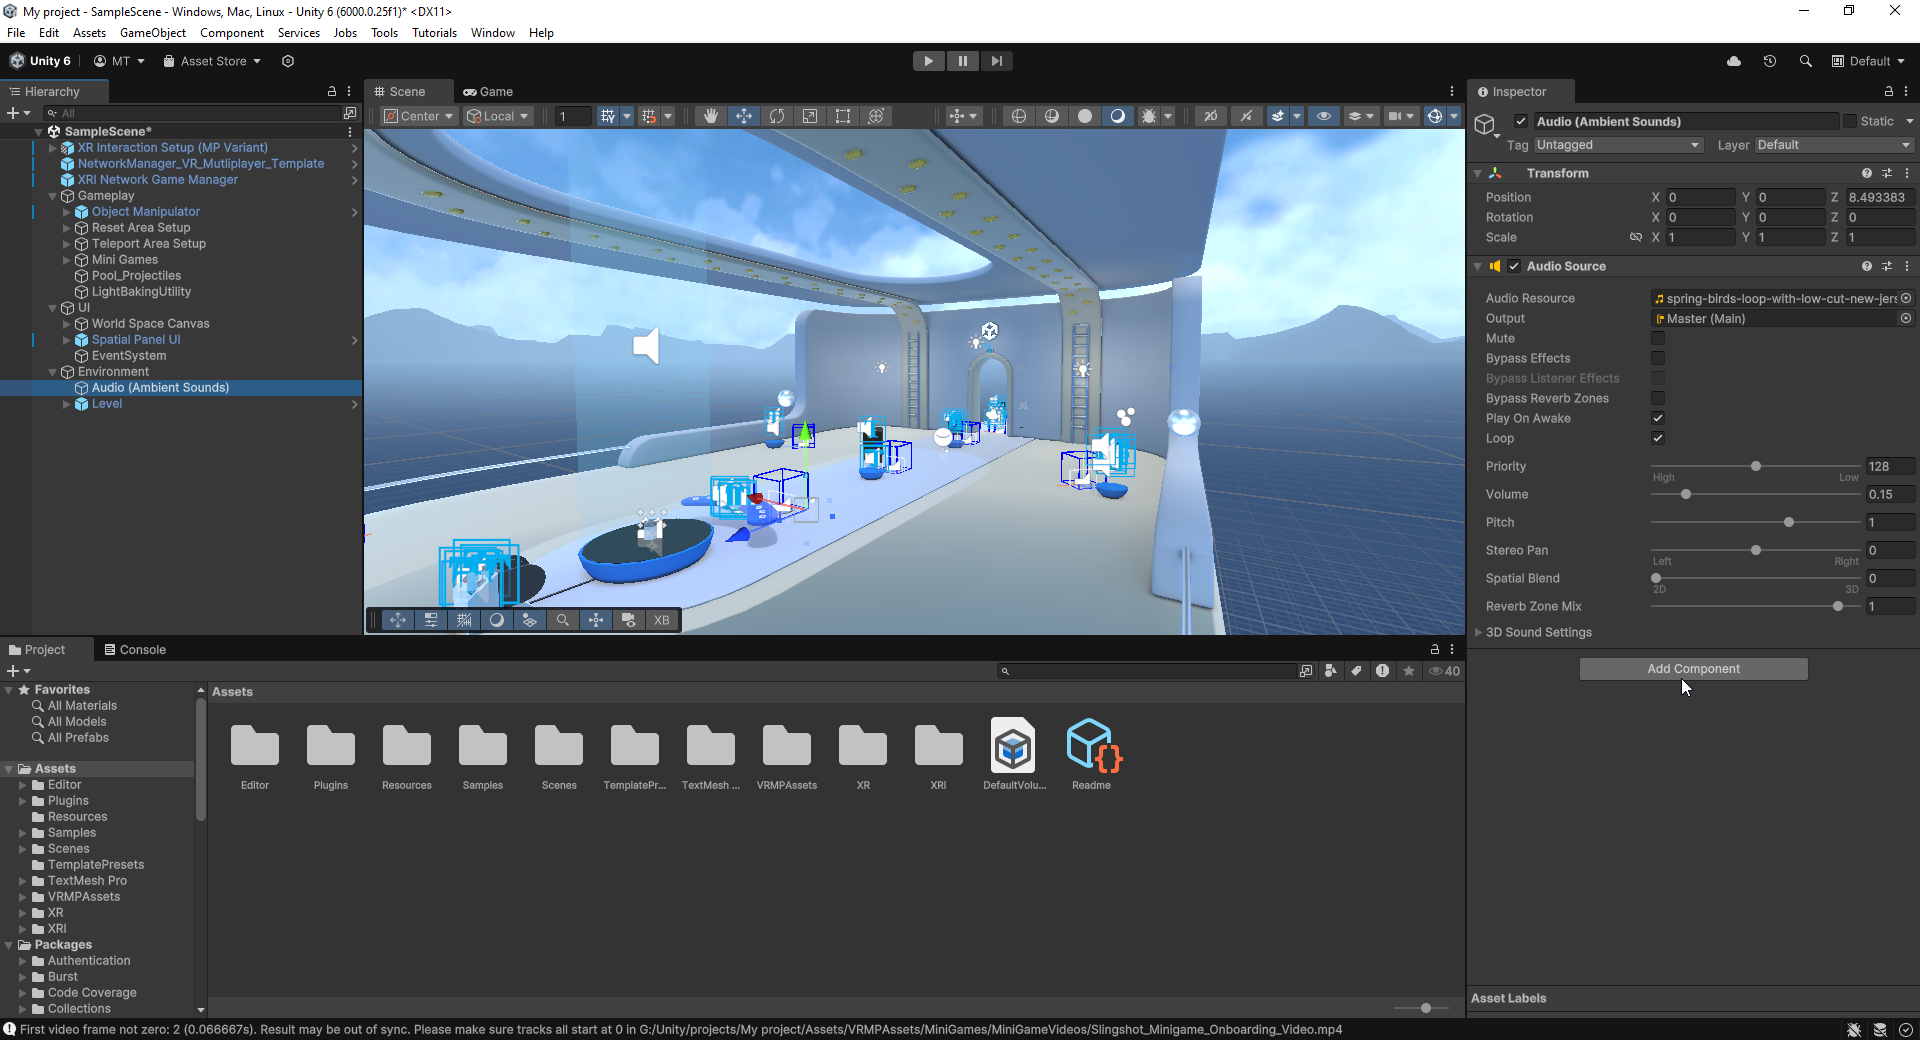
\includegraphics[width=0.8\textwidth]{obrazky/unity_hlavni.png}
	\caption{Unity hlavní okno}
	\label{fig:unity_hlavni_okno}
\end{figure}

Programovat v Unity můžeme buď za pomocí vizuálního programování, viz obr.\ref{fig:unity_vizualni}, či za pomocí tradičního programování v jazyce C\#.

\begin{figure}[H]
	\centering
	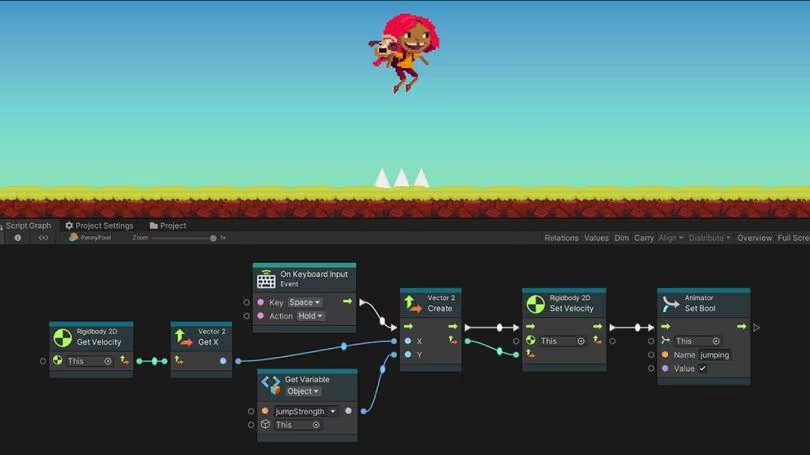
\includegraphics[width=0.8\textwidth]{obrazky/unity_vizualni_programovani.png}
	\caption{Unity vizuální programování}
	\label{fig:unity_vizualni}
\end{figure}
Pro vytvoření skriptu stačí kliknout na požadovaný objekt, v pravém panelu najít tlačítko "Add Component" a v tomto submenu najít možnost "New script", viz obr.\ref{fig:unity_novy_skript}.

Po pojmenování nového skriptu ho nalezneme v souboru Assets, odkud ho můžeme rozkliknout a otevřít pro editování v externím editoru, nikoliv v Unity. 

\begin{figure}[H]
	\centering
	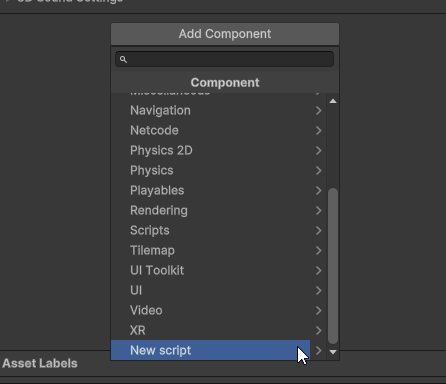
\includegraphics[width=0.8\textwidth]{obrazky/unity_pridani_skript.png}
	\caption{Submenu pro přidání skriptu k objektu}
	\label{fig:unity_novy_skript}
\end{figure}

Při vytvoření skriptu touto metodou se nám zobrazí již předgenerovaná "kostra" skriptu, se kterou můžeme následovně pracovat, viz obr.\ref{fig:unity_skript}.

\begin{figure}[H]
	\centering
	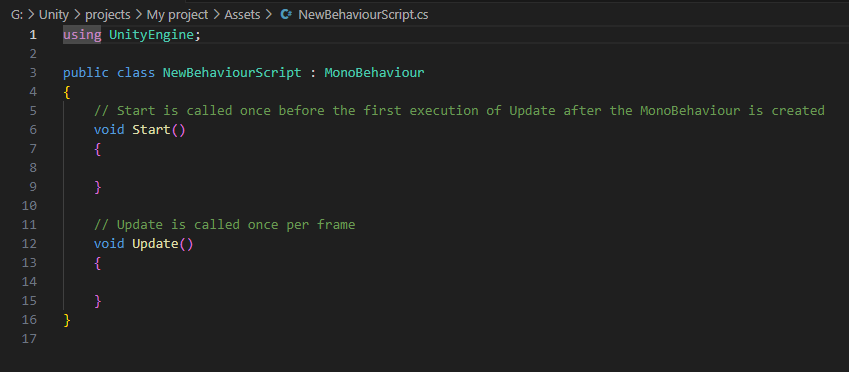
\includegraphics[width=0.8\textwidth]{obrazky/unity_skript_kostra.png}
	\caption{Nový skript po vytvoření pomocí Add Component}
	\label{fig:unity_skript}
\end{figure}


\chapter{Mřížková Boltzmannova metoda}

\chapter{Návrh a implementace programu}
\section{Postup při návrhu}


\section{Technické detaily implementace}

\chapter*{Závěr}
\addcontentsline{toc}{chapter}{Závěr} % SEM NESAHEJTE!
%
Zde napište text závěru své práce (1-3 strany, nerozdělujte na podkapitoly) nebo jej vložte ze samostatného souboru: např. příkazem \texttt{\textbackslash input\{vnitrek\_zaver.tex\}}. \par Závěr by měl obsahovat shrnutí práce a~zopakovat/zdůraznit, jaké jsou výsledky. Může obsahovat i~náměty na budoucí rozšířené práce. \par V~závěru práce byste neměli hodnotit svou práci -- to udělají členové komise při státní závěrečné zkoušce.
%
%\input{vnitrek_zaver.tex}










%%%%%%%%%%%% SEZNAM POUŽITÝCH ZDROJŮ (LITERATURA) %%%%%%%%%%%%
\clearpage
\addcontentsline{toc}{chapter}{Seznam použitých zdrojů} % SEM NESAHEJTE!
\begin{thebibliography}{99}   
% následující text (2 řádky) zaměňte citacemi svých zdrojů

\bibitem{htcvive}
HTC. \textit{HTC Vive} [online]. 2016 [cit. 2024-11-03]. Dostupné z: https://www.vive.com/us/

\bibitem{valveindex}
VALVE CORPORATION. \textit{Valve Index} [online]. 2019 [cit. 2024-11-03]. Dostupné z: https://store.steampowered.com/valveindex

\bibitem{EhojVv10CLuHHXEX}
VALVE CORPORATION. \textit{Half-Life: Alyx} [online]. 2020 [cit. 2024-11-10]. Dostupné z: https://store.steampowered.com/app/546560/HalfLife\_Alyx/

\bibitem{metaquest}
META. \textit{Meta Quest} [online]. 2020 [cit. 2024-11-03]. Dostupné z: https://www.meta.com/quest/quest-pro/

\bibitem{unityvr}
UNITY TECHNOLOGIES. \textit{Unity VR OpenXR} [online]. 2024 [cit. 2024-11-03]. Dostupné z: https://docs.unity3d.com/Packages/com.unity.xr.openxr@1.13/manual/index.html

\bibitem{unityvrdokovladani}
UNITY TECHNOLOGIES. \textit{Unity VR dokumentace ovládání} [online]. 2024 [cit. 2024-11-03]. Dostupné z: https://docs.unity3d.com/560/Documentation/Manual/OpenVRControllers.html

\bibitem{unrealvr}
EPIC GAMES. \textit{Unreal Engine XR} [online]. 2024 [cit. 2024-11-03]. Dostupné z: https://www.unrealengine.com/en-US/xr

\bibitem{unityvr_dalsi}
UNITY TECHNOLOGIES. \textit{Unity VR} [online]. 2024 [cit. 2024-11-03]. Dostupné z: https://unity.com/solutions/vr

\bibitem{precisionos}
EPIC GAMES. \textit{Precision OS} [online]. 2020 [cit. 2024-11-03]. Dostupné z: https://www.unrealengine.com/en-US/spotlights/vr-medical-simulation-from-precision-os-trains-surgeons-five-times-faster

\bibitem{virtamed}
VIRTAMED AG. \textit{Virtamed simulace} [online]. 2024 [cit. 2024-11-03]. Dostupné z: https://www.virtamed.com/en/custom-solutions/virtual-reality

\bibitem{unityvrstavebnictvi}
UNITY TECHNOLOGIES. \textit{Unity VR case study stavebnictví} [online]. 2017 [cit. 2024-11-03]. Dostupné z: https://unity.com/case-study/outhere-and-skanska

\bibitem{paraviewvrdok}
KITWARE. \textit{ParaView VR dokumentace} [online]. 2024 [cit. 2024-11-03]. Dostupné z: https://www.kitware.com/navigation-basics-in-virtual-reality-with-paraview/

\bibitem{nvidiaindexdok}
NVIDIA. \textit{NVIDIA IndeX dokumentace} [online]. 2024 [cit. 2024-11-03]. Dostupné z: https://catalog.ngc.nvidia.com/orgs/nvidia-hpcvis/containers/paraview-index

\bibitem{nvidiaindex}
NVIDIA. \textit{NVIDIA IndeX} [online]. 2024 [cit. 2024-11-03]. Dostupné z: https://developer.nvidia.com/index

\bibitem{unrealvrdok}
EPIC GAMES. \textit{Unreal Engine XR dokumentace} [online]. 2024 [cit. 2024-11-03]. Dostupné z: https://dev.epicgames.com/documentation/en-us/unreal-engine/developing-for-xr-experiences-in-unreal-engine?application\_version=5.4

\bibitem{openvrdok}
VALVE CORPORATION. \textit{OpenVR} [online]. 2024 [cit. 2024-11-03]. Dostupné z: https://github.com/ValveSoftware/openvr


\bibitem{unitypodpora}
UNITY TECHNOLOGIES. \textit{Unity VR podpora} [online]. 2024 [cit. 2024-11-03]. Dostupné z: https://docs.unity3d.com/560/Documentation/Manual/VRDevices-OpenVR.html


\bibitem{unityxrinteract}
UNITY TECHNOLOGIES. \textit{Unity XR interaction toolkit} [online]. 2024 [cit. 2024-11-03]. Dostupné z: https://docs.unity3d.com/Packages/com.unity.xr.interaction.toolkit@2.3/manual/index.html

\bibitem{unityvrdok}
UNITY TECHNOLOGIES. \textit{Unity VR dokumentace} [online]. 2024 [cit. 2024-11-03]. Dostupné z: https://docs.unity3d.com/Manual/VROverview.html

\bibitem{unitymulti}
UNITY TECHNOLOGIES. \textit{Unity multiplatform} [online]. 2024 [cit. 2024-11-03]. Dostupné z: https://unity.com/solutions/multiplatform

\bibitem{paraviewscript}
KITWARE. \textit{ParaView scripting} [online]. 2024 [cit. 2024-11-03]. Dostupné z: https://www.paraview.org/scripting/
\end{thebibliography}
% formát: ČSN ISO 690. Můžete si to vygenerovat na http://www.citacepro.com (přihlaste se přes odkaz "ČVUT"), umí to vygenerovat TeX
% řazení: abecedně podle autora (resp. provního slova, není-li znám autor)


%%%%%%%%%%%% PŘÍLOHY PRÁCE %%%%%%%%%%%%
\newpage % SEM NESAHEJTE!
\addcontentsline{toc}{chapter}{Přílohy} % SEM NESAHEJTE!
\appendix % SEM NESAHEJTE!


%%%%%%%%%%%% Příloha A (tj. 1. kapitola v rámci příloh) %%%%%%%%%%%%
\chapter{Dokumentace k aplikaci} % zde změňte název přílohy, příp. zakomentujte a vložte soubor, kde je název přílohy + její text (odmažte/zakomentujte text níže + odkomentujte \input{}):
%Zde napište text první přílohy nebo jej vložte, např.: \texttt{\textbackslash input\{priloha\_A.tex\}}.
%
%\input{priloha_A.tex} % text vkládán ze souboru, kde je i příkaz \chapter{...}


\end{document} % SEM NESAHEJTE! Konec.
